\chapter{Dari Biji Menjadi Tumbuhan}\label{ch:g2:from-seed-to-plant}

Guncangkan sebuah polong kacang yang kering, dan butir-butir kacang
yang keras berjatuhan --- kering, kusam, tampaknya tak bernyawa
seperti kerikil. Namun tanamlah satu di dalam tanah lalu siram, dan
dalam beberapa hari sesuatu yang luar biasa terjadi di bawah
permukaan. Satu \omterm{def:g1:plants-around-us:plant}{tumbuhan} utuh terlipat di dalamnya, menanti isyaratnya.

\section{Apa itu biji}

\begin{definition}[Biji]\label{def:g2:from-seed-to-plant:seed}
Suatu \emph{biji}\index{biji} adalah permulaan sebuah \omterm{def:g1:plants-around-us:plant}{tumbuhan} baru,
yang dibuat oleh \omterm{def:g1:plants-around-us:plant}{tumbuhan} induknya. Di dalam kulit bijinya yang melindunginya,
sebutir biji menyimpan:
\begin{itemize}
  \item sebuah \omterm{def:g1:plants-around-us:plant}{tumbuhan} mungil yang sudah dimulai --- yaitu
        \emph{lembaga}\index{lembaga} \omterm{def:g1:plants-around-us:plant}{tumbuhannya}, dengan bakal \omterm{def:g1:plants-around-us:parts}{akar}
        dan bakal tunas;
  \item cadangan makanan untuk memberinya makan sampai ia dapat makan
        sendiri.
\end{itemize}
\end{definition}

\begin{example}[Membuka kacang yang direndam]\label{ex:g2:from-seed-to-plant:open}
Rendam sebutir kacang putih yang besar semalaman, dan kulit bijinya
terlepas dengan mudah. Kacangnya terbuka menjadi dua belahan yang
tebal --- cadangan makanannya --- dan di situ, terselip di salah satu
tepinya, terbaring sebuah \omterm{def:g1:plants-around-us:plant}{tumbuhan} pucat yang mungil, ujung \omterm{def:g1:plants-around-us:parts}{akar} dan
\omterm{def:g1:plants-around-us:parts}{daun} pertama yang terlipat, sekecil sebutir beras. \omterm{def:g1:plants-around-us:plant}{Tumbuhan} barunya
memang sudah ada di situ sejak semula.
\end{example}

\begin{omfigure}
\begin{tikzpicture}
  \node[anchor=south west, inner sep=0] (img) at (0,0)
    {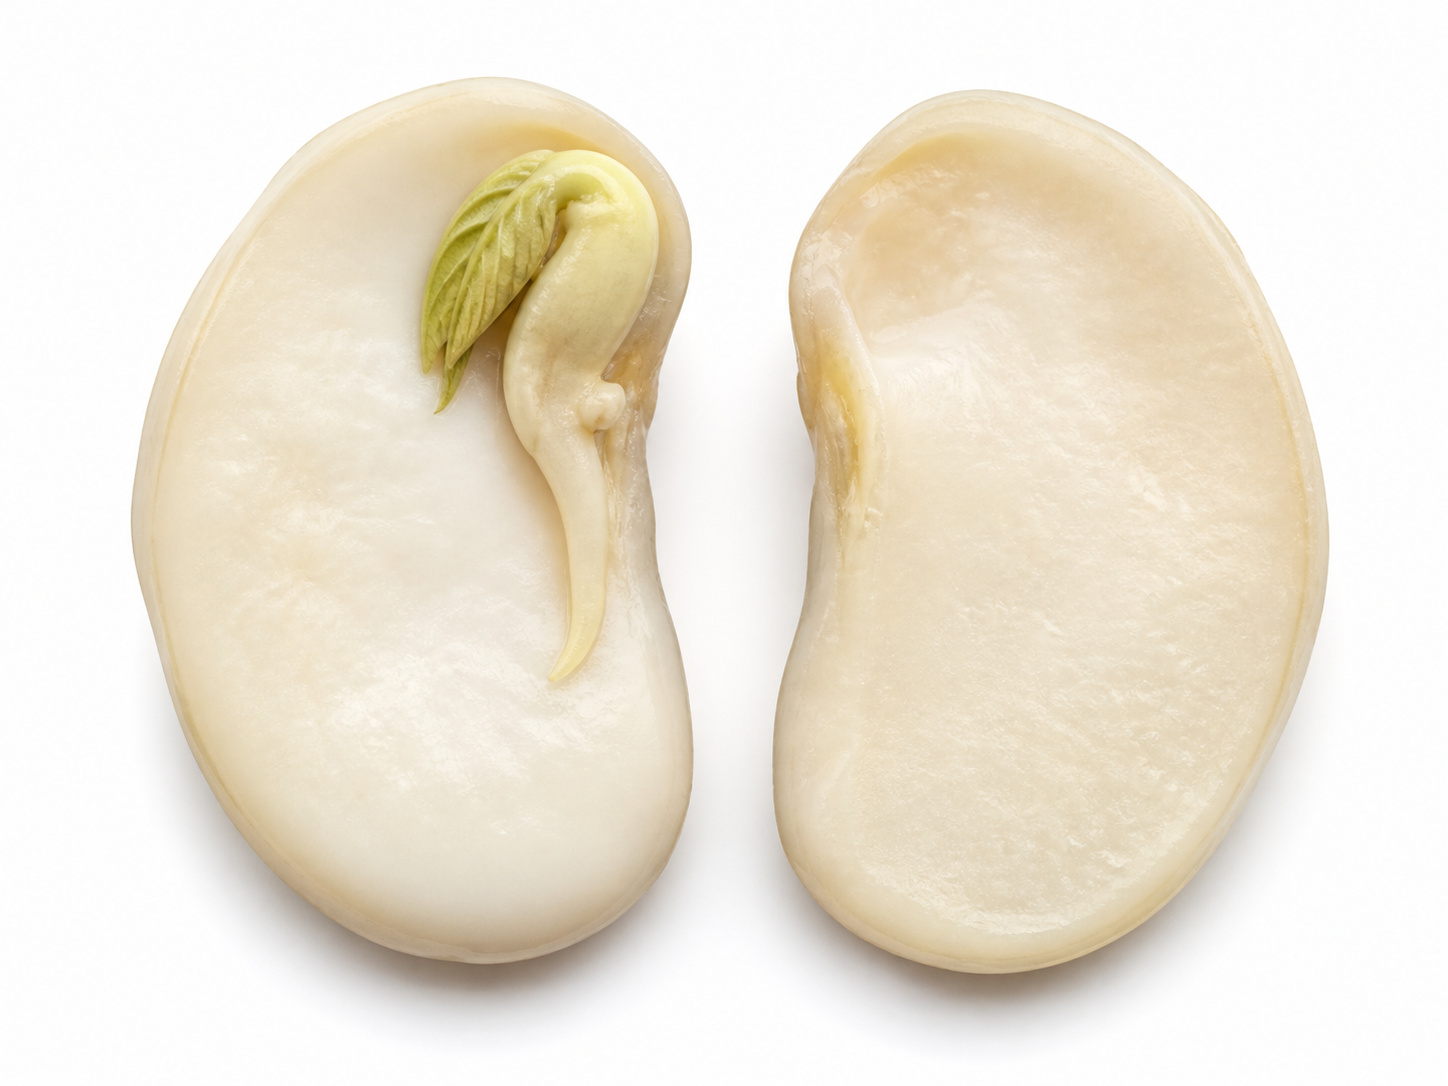
\includegraphics[width=0.62\linewidth]{images/book1/ai/fig-bean-open.png}};
  \begin{scope}[x={(img.south east)}, y={(img.north west)},
      every node/.style={font=\small}]
    \draw[omDef, thick] (0.35,0.79) -- (0.26,0.94)
      node[above] {daun pertama yang terlipat};
    \draw[omDef, thick] (0.40,0.38) -- (0.28,-0.04)
      node[below] {ujung akarnya};
    \draw[omDef, thick] (0.78,0.35) -- (0.80,-0.04)
      node[below, align=center] {dua belahan tebal:\\ cadangan makanannya};
  \end{scope}
\end{tikzpicture}

{\small Di dalam kacang yang telah direndam dan dibuka: sebuah
\omterm{def:g1:plants-around-us:plant}{tumbuhan} mungil --- ujung \omterm{def:g1:plants-around-us:parts}{akar} dan \omterm{def:g1:plants-around-us:parts}{daun} pertama yang terlipat ---
terbaring di samping cadangan makanannya.}
\end{omfigure}

\begin{remark}[Biji melintasi dapur kita]\label{rem:g2:from-seed-to-plant:kitchen}
Kacang, ercis, miju-miju, beras, \omterm{def:g2:from-seed-to-plant:seed}{biji} \omterm{def:g1:plants-around-us:parts}{bunga} matahari, \omterm{def:g2:from-seed-to-plant:seed}{biji} di dalam
apel dan \omterm{def:g2:from-seed-to-plant:seed}{biji} besar di dalam buah persik: dapur penuh dengan \omterm{def:g2:from-seed-to-plant:seed}{biji}.
Sebagian mungil, seperti \omterm{def:g2:from-seed-to-plant:seed}{biji} apiun; kelapa adalah \omterm{def:g2:from-seed-to-plant:seed}{biji} raksasa.
Masing-masing, kalau diberi kesempatan, akan berusaha menjadi
\omterm{def:g1:plants-around-us:plant}{tumbuhan}.
\end{remark}

\section{Perkecambahan}

\begin{definition}[Perkecambahan]\label{def:g2:from-seed-to-plant:germination}
Yang disebut \emph{perkecambahan}\index{perkecambahan} adalah saat
sebutir \omterm{def:g2:from-seed-to-plant:seed}{biji} terbangun lalu mulai tumbuh: ia membengkak oleh air,
kulit bijinya terbelah, \omterm{def:g1:plants-around-us:parts}{akar} kecilnya keluar lebih dahulu lalu menukik ke
bawah, kemudian tunasnya naik, membawa \omterm{def:g1:plants-around-us:parts}{daun} hijau pertamanya ke arah
cahaya. Kita katakan bahwa \omterm{def:g2:from-seed-to-plant:seed}{bijinya}
\emph{berkecambah}\index{berkecambah}.
\end{definition}

\begin{proposition}[Yang dibutuhkan biji untuk berkecambah]\label{prop:g2:from-seed-to-plant:needs}
Untuk \omterm{def:g2:from-seed-to-plant:germination}{berkecambah}, sebutir \omterm{def:g2:from-seed-to-plant:seed}{biji} membutuhkan \emph{air} dan
\emph{kehangatan}. Ia belum membutuhkan cahaya: cadangan makanannya
memberi makan \omterm{prop:g2:from-seed-to-plant:cycle}{kecambahnya} pada mulanya, bahkan di bawah tanah, dalam
gelap. Tanpa air, atau dalam keadaan dingin, \omterm{def:g2:from-seed-to-plant:seed}{biji} yang baik hanya
menunggu.
\end{proposition}
\admitted

\begin{example}[Mengapa menyemai menunggu musim semi]\label{ex:g2:from-seed-to-plant:spring}
Tukang kebun menyemai kacang pada musim semi, bukan pada musim dingin:
\omterm{def:g2:from-seed-to-plant:seed}{biji} di dalam tanah yang dingin akan menunggu --- atau membusuk ---
alih-alih \omterm{def:g2:from-seed-to-plant:germination}{berkecambah}. Hari yang hangat dan tanah yang disiram tepat
merupakan kedua isyarat pada
\cref{prop:g2:from-seed-to-plant:needs}.
\end{example}

\begin{method}[Menyemai biji dan mengamati perkecambahannya]\label{met:g2:from-seed-to-plant:sow}
\begin{enumerate}
  \item Lapisi sebuah toples kaca dengan kapas atau kertas yang lembap;
  \item selipkan sebutir kacang di antara kaca dan kapasnya, agar kamu
        dapat melihatnya;
  \item simpan toplesnya di ruangan yang hangat dan jaga kapasnya
        tetap lembap;
  \item amati setiap hari dan catat apa yang kamu lihat: membengkak,
        kulit bijinya terbelah, \omterm{def:g1:plants-around-us:parts}{akar} ke bawah, tunas ke atas.
\end{enumerate}
Kacanya membuat terlihat apa yang biasanya terjadi di bawah tanah.
\end{method}

\begin{omfigure}
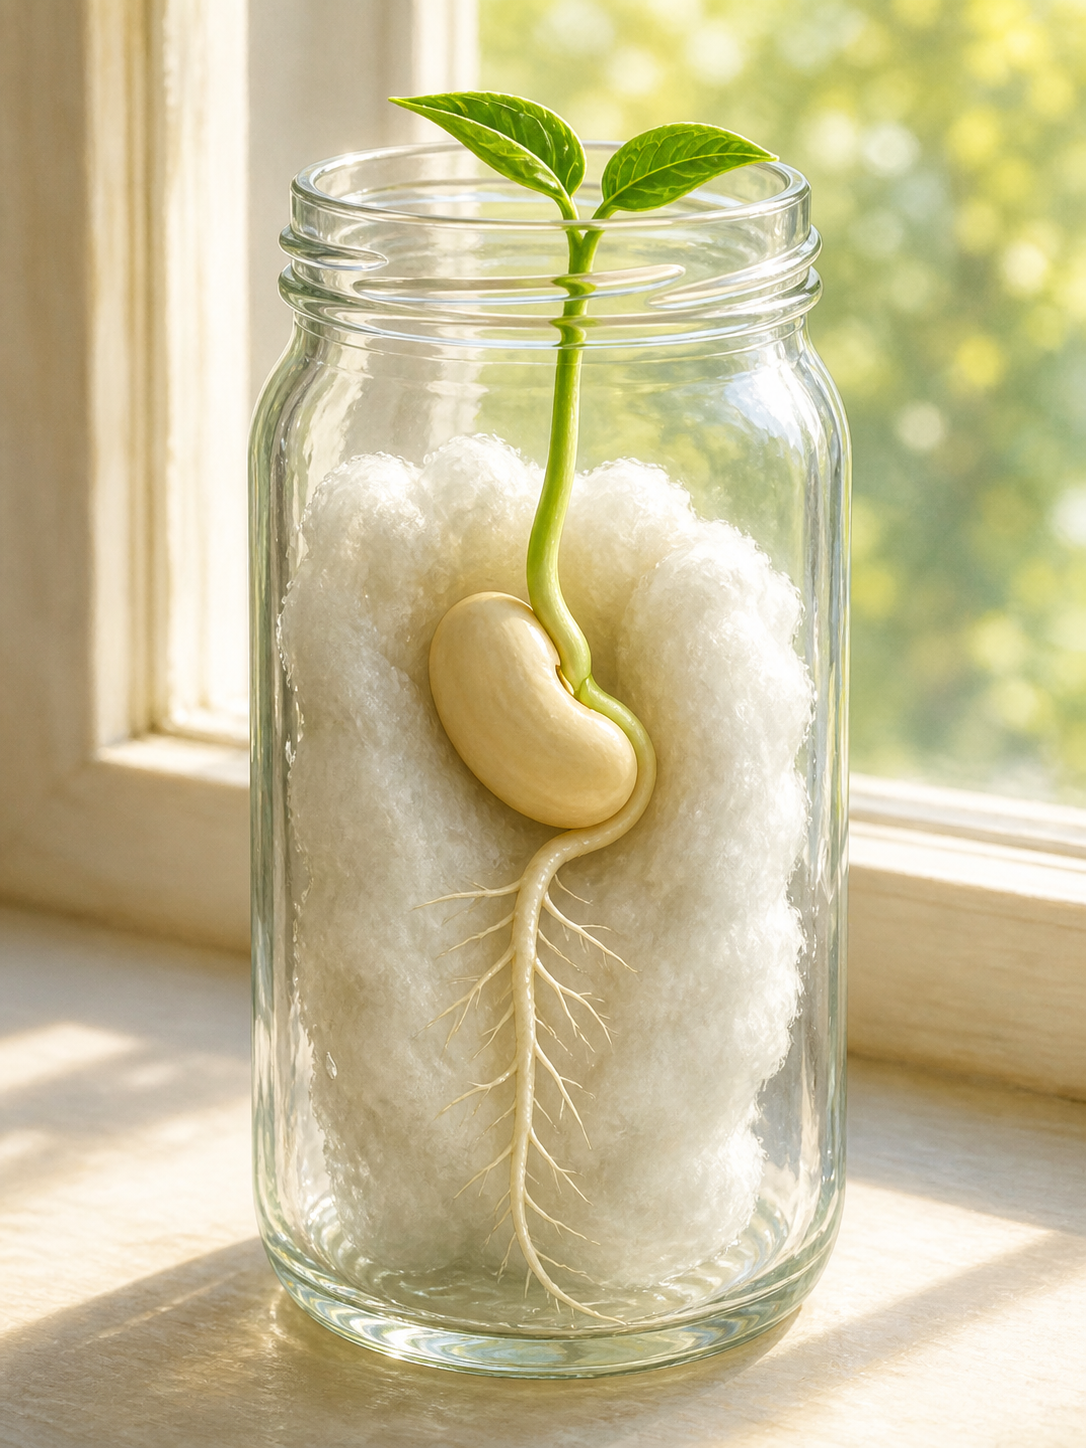
\includegraphics[width=0.44\linewidth]{images/book1/ai/g2-seed-bean-jar.png}

{\small Percobaan toples di tengah \omterm{def:g2:from-seed-to-plant:germination}{perkecambahan}: \omterm{def:g1:plants-around-us:parts}{akar} ke bawah,
tunas ke atas, dan \omterm{def:g2:from-seed-to-plant:seed}{bijinya} yang mengosong di antara keduanya.}
\end{omfigure}

\begin{remark}[Akar ke bawah, tunas ke atas --- selalu]\label{rem:g2:from-seed-to-plant:updown}
Bagaimanapun kacangnya terbaring di dalam toples --- miring, terbalik
--- \omterm{def:g1:plants-around-us:parts}{akarnya} selalu berbelok ke bawah dan tunasnya selalu berbelok ke
atas. \omterm{prop:g2:from-seed-to-plant:cycle}{Kecambahnya} tidak dapat melihat, namun ia tahu ke mana arah
atas. \omterm{def:g1:plants-around-us:plant}{Tumbuhan} mengindera lebih banyak daripada yang diperlihatkannya.
\end{remark}

\section{Dari kecambah menjadi tumbuhan berbiji}

\begin{proposition}[Daur hidup tumbuhan]\label{prop:g2:from-seed-to-plant:cycle}
Sebuah \emph{kecambah}\index{kecambah} tumbuh menjadi \omterm{def:g1:plants-around-us:plant}{tumbuhan}
yang berakar, berbatang dan berdaun; \omterm{def:g1:plants-around-us:plant}{tumbuhannya} berbunga; \omterm{def:g1:plants-around-us:parts}{bunganya} membuat
\emph{\omterm{def:g2:from-seed-to-plant:seed}{biji}} baru; dan daurnya dapat bermula lagi. Satu tanaman kacang
saja dapat membuat berlusin-lusin kacang baru dalam satu musim panas.
\end{proposition}
\admitted

\begin{example}[Satu kacang, satu musim panas]\label{ex:g2:from-seed-to-plant:summer}
Disemai pada bulan Mei, sebutir kacang \omterm{def:g2:from-seed-to-plant:germination}{berkecambah} dalam seminggu;
menjelang Juni ia sudah menjadi tanaman berdaun lebat yang memanjat
tiangnya; pada bulan Juli datang \omterm{def:g1:plants-around-us:parts}{bunga-bunga} putih, lalu polong hijau;
pada bulan Agustus polongnya menggantung berat, masing-masing memuat
sederet kacang baru --- \omterm{def:g2:from-seed-to-plant:seed}{biji} untuk tahun depan, yang dibuat oleh
tanaman tahun ini.
\end{example}

\section{Latihan}

\begin{exercise}[$\star$]\label{exo:g2:from-seed-to-plant:1}
Dua hal apa yang terbaring di dalam kulit biji sebutir kacang?
\end{exercise}

\begin{exercise}[$\star$]\label{exo:g2:from-seed-to-plant:2}
Apa arti \emph{\omterm{def:g2:from-seed-to-plant:germination}{berkecambah}}? Apa yang keluar lebih dahulu dari
\omterm{def:g2:from-seed-to-plant:seed}{bijinya}: \omterm{def:g1:plants-around-us:parts}{akarnya}, atau tunasnya?
\end{exercise}

\begin{exercise}[$\star$]\label{exo:g2:from-seed-to-plant:3}
Sebutkan dua hal yang dibutuhkan sebutir \omterm{def:g2:from-seed-to-plant:seed}{biji} untuk \omterm{def:g2:from-seed-to-plant:germination}{berkecambah}.
Kebutuhan terkenal \omterm{def:g1:plants-around-us:plant}{tumbuhan} dewasa yang mana yang \emph{tidak} ada
dalam daftar itu?
\end{exercise}

\begin{exercise}[$\star$]\label{exo:g2:from-seed-to-plant:4}
Bagaimana \omterm{prop:g2:from-seed-to-plant:cycle}{kecambah} yang terkubur dapat tumbuh dalam gelap, sebelum
mencapai cahaya? Dari mana makanannya berasal pada mulanya?
\end{exercise}

\begin{exercise}[$\star$]\label{exo:g2:from-seed-to-plant:5}
Sebutkan empat jenis \omterm{def:g2:from-seed-to-plant:seed}{biji} yang dapat kamu temukan di dapur.
\end{exercise}

\begin{exercise}[$\star$]\label{exo:g2:from-seed-to-plant:6}
Mengapa tukang kebun menyemai pada musim semi dan bukan musim dingin?
\end{exercise}

\begin{exercise}[$\star$]\label{exo:g2:from-seed-to-plant:7}
Urutkan: polong berisi kacang baru --- \omterm{def:g2:from-seed-to-plant:seed}{biji} --- \omterm{def:g1:plants-around-us:plant}{tumbuhan} berbunga ---
\omterm{prop:g2:from-seed-to-plant:cycle}{kecambah} --- tanaman berdaun lebat.
\end{exercise}

\begin{exercise}[$\star$]\label{exo:g2:from-seed-to-plant:8}
Cobalah: siapkan toples kaca pada \cref{met:g2:from-seed-to-plant:sow}
dengan dua butir kacang --- satu terbaring miring, satu terbalik.
Sesudah \omterm{def:g2:from-seed-to-plant:germination}{berkecambah}, bandingkan \omterm{def:g1:plants-around-us:parts}{akar} dan tunasnya. Apa yang diramalkan
\cref{rem:g2:from-seed-to-plant:updown}?
\end{exercise}

\begin{exercise}[$\star\star$]\label{exo:g2:from-seed-to-plant:9}
Nina menyimpan sebungkus \omterm{def:g2:from-seed-to-plant:seed}{biji} kacang di laci yang kering selama satu
tahun penuh, dan \omterm{def:g2:from-seed-to-plant:seed}{biji} itu tetap \omterm{def:g2:from-seed-to-plant:germination}{berkecambah} ketika akhirnya ia semai.
Mengapa \omterm{def:g2:from-seed-to-plant:seed}{biji} itu tidak tumbuh dan juga tidak mati di dalam laci? Pakai
\cref{prop:g2:from-seed-to-plant:needs}.
\end{exercise}

\begin{exercise}[$\star\star$]\label{exo:g2:from-seed-to-plant:10}
Anak ayam pada \cref{ch:g2:animals-grow-up} tumbuh di dalam \omterm{def:g2:animals-grow-up:born}{telurnya},
diberi makan oleh kuning telurnya. Apa yang memainkan peran kuning
telur di dalam sebutir kacang? Apa persamaan sebutir \omterm{def:g2:animals-grow-up:born}{telur} dan sebutir
\omterm{def:g2:from-seed-to-plant:seed}{biji}?
\end{exercise}
